\documentclass[a4paper, 12pt, twoside]{article}
\usepackage{ae,aecompl}
\usepackage[T1]{fontenc}
\usepackage[utf8]{inputenc}
\usepackage{textcomp}
\usepackage{anysize}
% left right up down
\marginsize{3.2cm}{2.8cm}{2cm}{2cm}
\usepackage{setspace}
\setstretch{1.2}
\frenchspacing
\usepackage{chemfig}
\usepackage{gensymb}
\usepackage{fancyhdr}
\usepackage{enumerate}
\usepackage{amsmath}
\usepackage{upgreek}
\usepackage{indentfirst}
\usepackage{sidecap}
\numberwithin{equation}{section}
\numberwithin{figure}{section}
\numberwithin{table}{section}
\usepackage{multicol}
\usepackage{float}
\setcounter{tocdepth}{1}
\pagestyle{empty}
% uncomment for hyperlinks
\usepackage{xcolor}
\usepackage[colorlinks = true,
            linkcolor = red,
            urlcolor  = blue,
            citecolor = blue,
            anchorcolor = blue]{hyperref}



\title{Physical chemistry laboratory practice}
\author{\emph{written by:} \\ Barna Kovács \\ Sándor Kunsági-Máté \\ András Kiss \\ Géza Nagy \\ \\ \emph{translated by:} \\ András Kiss \\ Katalin Ősz \\ Gábor Lente\\ \\ \\ \\ \\ \\
\includegraphics[width=0.2\textwidth]{fig/pte_logo.eps} \\
Department of General and Physical Chemistry \\ University of Pécs}

\begin{document}

\clearpage\maketitle
\thispagestyle{empty}
\newpage 
\tableofcontents
\newpage

\section{Foreword}

Today, automatization of measurements seems to reduce the role of human operators in a lot of areas of science and industry. To understand and improve these methods, however, a closer interaction with the measured phenomena is necessary. It is the authors' hope that these practices will help students to understand the fundamental aspects of measurements in physical chemistry, and the derivation of important parameters from recorded data in general.

This handout is primarily written for the physical chemistry laboratory practice of Chemistry BSc. and pharmacy students. In each practice, you will measure physical and chemical properties, and then use basic relationships in physical chemistry to calculate important parameters such as heat of dissolution, rate constant, pK, selectivity coefficient of ion-selective electrodes, and others.

During the course, the you will familiarize yourself with basic and intermediate level methods in physical chemical measurements. The authors however, assume a basic knowledge of general and analytical chemistry, regarding simple concentration calculations, titrimetric methods, basic electrochemistry, and photometric methods.

The effort on each practice should be divided into three more or less equal parts. First, it is essential for a successful practice to prepare in advance. Second, the practice itself should be carried out with great care and precision. Good laboratory practice (GPL) is advised for all students, and regardless of the topic. And third, a laboratory notebook should be prepared during, and finished after the practice to make it complete with the necessary calculations, figures, and conclusions.

The authors wish a successful course for each student undertaking these practices and hope to contribute to their laboratory skills and their understanding of physical chemistry.

\vspace{2 cm}

Pécs, 2018 December \hfill The authors

\newpage
\input{tex_en/drug_decomposition.tex}
\newpage
\clearpage
\input{tex_en/ion_selective.tex}
\newpage
%\setcounter{section}{1}
\section{Bestimmung des Dissoziationskonstanten von schwachen Säuren mit Leitfähigkeitsmessung}
\subsection{Theoretische Grundlage}

Elektrischer Widerstand ist eine Eigenschaft des Materials. Nach dem ohmschen Gesetz ist zwischen den Materialen durchpliessenden Stromstärke ($I$) und den Strom erstellenden Spannung ($U$) ein gerades Verhältniss.


\begin{equation}
\label{eq:ohm}
	U
	=
	I
	\cdot
	R
\end{equation}

wo der Verhältnissfaktor $R$ als Widerstand des Materials genannt wird, dessen Einheit ist der ohm ($\ohm$).
An spezifischer Widerstand verstehen wir den Quotient von der Spannung die zur Erstellung von ein 1 A (Amper) starken Strom nötig ist und den Strom von 1 A. %%%

In der Elektrochemie ist es aus mehreren Hinsichten bevorzüglich, wenn wir den Reziprok von oben genannten Einheiten benutzen: den Reziprok vom Widerstand nennen wir Leitfähigkeit (Enheit ist Siemens, S$ = 1 / \ohm$), den Reziprok von spezifischen Widerstand nennen wir spezifischen Leitfähigkeit (Einheit ist S/cm).
An spezifischen Leitfähigkeit von Elektrolytlösungen ($\kappa$) nennen wir die Leitfähigkeit von Elektrolytlösung zwischen zwei Leitern von erste Klasse die 1 cm entfernt von einander sind und eine Fläche von 1 cm$^2$ haben.
Die spezifische Leitfähigkeit ist abhängig von der materiellen Qualität, von der Konzentration und von der Temperatur des Elektrolyten.
An molar spezifische Leitfähigkeit ($\Lambda _m$) verstehen wir den Quotient von der spezifischer Leitfähigkeit und der Konzentration.

\begin{equation}
\label{eq:lambdam}
        \Lambda_m
        =
        \frac
		{\kappa 1000 }
		{c}
	=
	\kappa V
\end{equation}

wo $c$ ist Konzentration (mol$\cdot$dm$^{-3}$), und $V$ ist Verdünnung.

Die molare Leitfähigkeit der unendlich verdünnten Lösung wird molare Grenzleitfähigkeit genannt ($\Lambda _m^0$).
Nach \emph{Kohlrausch}\footnote{Friedrich Wilhelm Georg Kohlrausch war ein deutscher Physiker und Physikochemiker.} summiert sich die Leitfähigkeit von Anionen und Kationen in dünnen Lösungen von starken Elektrolyten. 

%Kohlrausch szerint erős elektrolitok híg oldataiban az anionok és kationok moláris fajlagos vezetőképessége összeadódik.

\begin{equation}
\label{eq:kohlrausch2}
	\Lambda _m^0
	=
	\lambda _a^0 \nu _a z_a + \lambda _k^0 \nu _k z_k
%	/1000
\end{equation}

wo $z_a, z_k$ sind die Ladung, $\nu _a, \nu _k$ sind die stöchiometrischen Faktoren, und $\lambda _a^0, \lambda _k^0$ sind die Grenzleitfähigkeiten von Anionen ($a$) und Kationen ($k$).

Die Leitfähigkeit von dünnen Elektrolyten werden bezeichnet als:

\begin{equation}
\label{eq:lambdam}
        \lambda_c
        =
        \alpha
	\lambda_0
\end{equation}

wo $\alpha$ den Dissoziationsgrad, $\lambda _0$ die Grenzleitfähigkeit bedeutet.

Der Dissoziationskonstant einer schwachen Säure ist berechenbar wenn die Konzentrazion und der Dissoziationsgrad bekannt ist:

\begin{equation}
\label{eq:kd}
        K_d
        =
        \frac{\alpha^2 c}{1-\alpha}
\end{equation}

Es ist aber erwähnenswert, dass nach dem Debye--Hückel--Grenzgesetz, der Dissoziationkonstant $K_d$ bei konstanter Temperatur auch von Permittivität abhängig ist.

Wenn wir die nach $\alpha$ geordnete Form der Gleichung \ref{eq:lambdam} in die vorherige Gleichung substituieren, dann kommen wir auf den von \emph{Ostwald}\footnote{Friedrich Wilhelm Ostwald war ein deutsch-baltischer Chemiker und Philosoph.} bestimmten Zusammenhang der Dissoziation von schwachen Elektrolyten. Dieser Zusammenhang ist als \emph{Ostwaldsche Verdünnungsgesetz} bekannt:

\begin{equation}
\label{eq:ostwald}
        K_d
        =
        \frac{\lambda_c^2 c}{\lambda_0^2 - \lambda_0\lambda_c}
\end{equation}

Das bedeutet, dass wir dem K$_d$ mit Leitungsfähigeitsmessen bestimmen können.
$\lambda_c$ ist direkt messbar, wärend $\lambda_0$ mit der umgeordneten Form von Gesetz \ref{eq:ostwald} bestimmbar ist:

\begin{equation}
\label{eq:ostwald2}
        \frac{1}{\lambda_c}
        =
	\lambda_c
	c
	\frac{1}{K_d \lambda_0^2}
	+\frac{1}{\lambda_0}
\end{equation}

Wenn wir $1/\lambda_c$ als Funktion von $\lambda_c c$ ($= \kappa$) erzeichnen, bekommen wir eine Gerade mit ein Ordinatenabschnitt von $1/\lambda_0$. 
Wenn $\lambda_c$ und $\lambda_0$ bekannt ist, können wir auch den Wert $K_d$ bestimmen.
Bei der Ausführung der Messungen sind folgende Dingen zu beachten: 

\begin{enumerate}[(a)]
\item Neben der gelösten Substanz trägt das Lösungsmittel zur gemessenen Leitfähigkeit der Lösung bei.
Mit eine zugäblichen Messung bestimmen wir die Leitfähigkeit der Lösungsmittel ($G_{\text{Lösungsmittel}}$), und diesen Wert subtrahieren wir aus dem Leitfähigkeit der Lösung.

\item In der Praktik messen wir die Leitfähigkeit nicht mit dem Messgerät aus der Definition von spezifischen Leitfähigkeit, sondern mit einer einfacher, nutzbarer Zelle mit abweichender Geometrie.
Den Unterschied berücksichtigen wir mit der Kalibrationparameter genannt als Zellenkonstant $C$.
Der Zellenkonstant bezeichnet die Verbindung zwischen der Lösung mit einen bekannten spezifischen Leitfähigkeit ($\kappa_{ref}$) und mit der Messzelle gemessene Leitfähigkeit($G_{\text{gemessene}}$). Die Einheit von Zellenkonstant ist m$^{-1}$ oder cm$^{-1}$.

\begin{equation}
\label{eq:c}
	C
	=
	\kappa_{\text{ref}}/G_{\text{measured}}
\end{equation}

\end{enumerate}

Aufgrund dessen bekommen wir den Beitrag der Lösung zur Leitfähigkeit folgender Weise: $\kappa_{\text{korr}} = (G_{\text{Lösung}} - G_{\text{Lössungsmittel}})C$,
wo $\kappa_{\text{korr}}$ ist ein korrigierte Wert von der spezifischen Leitfähigkeit von gelösste Substanz durch den Zellenkonstant und durch die spezifischen Leitfähigkeit des Lösungsmittels. 
$C$ ist der Zellenkonstant, nicht zu verwechseln mit der Konzentration, was mit kleinem $c$ bezeichnet wird.
So bekommen wir die molare Leitfähigkeit der Lösung folgenderweise:

\begin{equation}
\label{eq:c}
        \lambda
        =
        \kappa_{korr}
	V
\end{equation}

wo $V$ verdünnung bedeutet.

\begin{figure}[h!]
\centering
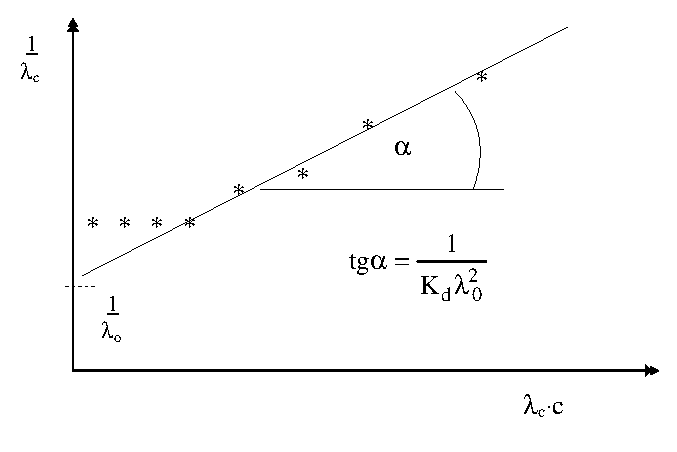
\includegraphics{fig/lambda0.eps}
\caption{Bestimmen der molaren Grenzleitfähigkeit ($\lambda_0$).}
\label{fig:}
\end{figure}

\subsection{Beschreibung des Praktikums}

Spülen Sie die Elektrode von Konduktometer (Leitfähigkeitsmessgerät) vier--fünfmal mit vollentzalztes Wasser, dann mit doppelentsalzten Wasser ($\kappa$ < 1 $\upmu$S/cm), was Sie von der technischen Hilfsperson bekommen.
Richten Sie eine Alkohollösung von 20 v/v\% Volumenkonzentration zu, mit dem Alkohol (Metanol, Etanol oder Propanol) was Ihnen der Praktikumleiter anbietet.
Richten Sie zweierlei Lösungen aus der bekommenen 1 mol$\cdot$dm$^{-3}$ Schwachsäure Stammlösung:
Nehmen Sie zwei trockene 100 cm$^3$ Messkolben und geben Sie mit der Pipette 2--2 cm$^3$ Stammlösung rein.
Dann füllen Sie den einen Messkolben mit doppelvollentsalztes Wasser, den anderen mit 20 v/v\% Alkohollösung bis zur Eichmarke.
Messen Sie die Leitfähigkeit in einen Messzylinder.
Füllen Sie erst die wasserverdünnte Lösung in den Messzylinder, und messen Sie die Leitfähigkeit.
Nachdem saugen Sie 25 cm$^3$ aus dieser Lösung und entlehren Sie sie in einen 50 cm$^3$ grossen Messkolben und füllen Sie bis zur Eichmarke mit doppelvollentsalztes Wasser.
Nach der sorgfeltigen Spülung der Elektrode, wiederholen Sie die Messungen.
Die Prozedur (Verdünnung, Spülung, Messung) wiederholen Sie noch dreimal--viermal.
Wiederholen Sie die ganze Prozedur mit den alkoholverdünnten Lösungen genauso, durch Spülung und Verdünnung mit Alkohollösung.

Bei jeder Messung notieren Sie die Temperatur der Lösung, was das Messgerät anzeigt.

Letzendlich, messen Sie die Leitfähigkeit von dem gebrauchten entzaltzten Wasser, und dem Alkohollösung vomit Sie die Messergäbniste korrigieren müssen.
Nachdem messen Sie die Leitfähigkeit von 0.1 oder 0.01 M KCl Lösung, damit Sie den Zellenkonstant bestimmen.

Abbildung \ref{fig:vez} zeigt das Schema von dem Leitfähigkeitsmesszellen.
In die Lösung tauchen wir zwei geometrischrichtig definierte indifferente Elektroden, und messen die entstehende Spannung. 
Um die elektrische Polarisation zu vermeiden, benutzt das Messgerät Wechselstrom. 

\begin{figure}
\centering
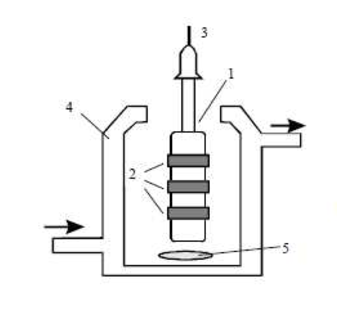
\includegraphics{fig/cond.eps}
\caption{Schema von dem Leitfähigkeitmesszellen. 1 - Elektroden, 2 - Platinum, 3 - elektrische Verbindung, 4 - doppelwandiger Behälter, 5 - Magnetrührer.}
\label{fig:vez}
\end{figure}

\subsection{Auswertung der Messungen}

\begin{enumerate}
\item Rechnen Sie der Zellenkonstant.
Die Messergäbnisse fassten Sie in eine Tabelle:

\begin{table}[!h]
\centering
\begin{tabular}{|c|c|c|c|c|c|c|c|}
\hline
c (mol $\cdot$ dm$^{-3}$) & G$_{\text{gemessene}}$ & $\kappa_{\text{korr}}$ (S $\cdot$ cm$^{-1}$) & $\lambda_c$ & $1/\lambda_c$ & $\lambda_c c$ & $\alpha$ & $K_d$ \\
\hline
... & ... & ... & ... & ... & ... & ... & ... \\
\end{tabular}
\label{table:vez}
\end{table}

\item Bestimmen Sie grafisch den $\lambda_0$ Wert. Mit diesem bekommenen Ergebnissen ($\lambda_c, \lambda_0$) rechnen Sie die $\alpha$ und $K_d$ auf jede Konzentration. 

\end{enumerate}

\newpage
\input{tex_en/vit_c.tex}
\newpage
\input{tex_en/sucrose_inversion.tex}
\newpage
\fancyhead[LE,RO]{Langmuir isotherm of a solid adsorbent}
\fancyhead[LO,RE]{\thesection}
\fancyfoot[LE,RO]{\thepage}
\fancyfoot[RE,LO]{\emph{Physical chemistry lab. practice for pharmacy students}}

%\setcounter{section}{7}
\section{Using the Langmuir isotherm to calculate the maximal adsorption capacity of a solid adsorbent}
\subsection{Introduction}

Adsorption is a physicochemical process, during which atoms, ions or molecules adhere to a surface.
The result is a thin layer of the adsorbate that is formed on the adsorbent surface (Fig. \ref{fig:adsorption}).
\begin{SCfigure}[][b]
\centering
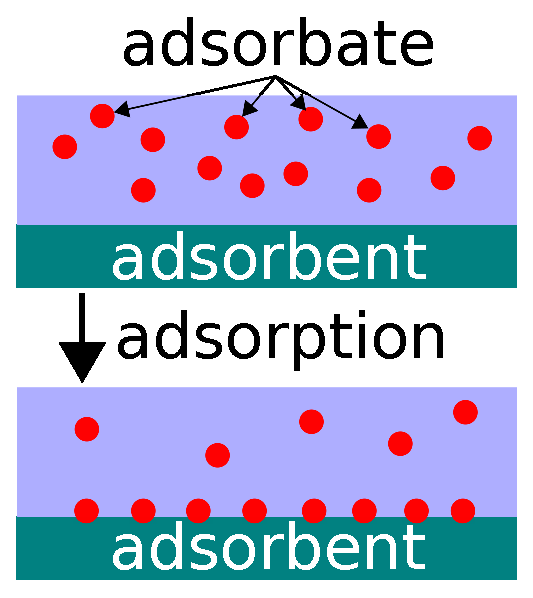
\includegraphics[width=0.25\textwidth]{adsorption.eps}
\caption{During adsorption, a thin adhered layer of the adsorbate is produced on the surface of the adsorbent.}
\label{fig:adsorption}
\end{SCfigure}
The original media from which the adsorbate originates can be gas or liquid.
The reverse process is called desorption.
Adsorption is an important process, and it is present in many areas of everyday life, industry, research, pharmacy.
It is an important step -- among many -- in heterogeneous catalysis, water treatment, removal by activated carbon.
Adsorption by activated carbon is used to remove toxins or unwanted dangerous substances from the gastrointestinal tract after poisonings.
Adsorption can be used in pharmaceutical industry to modulate the rate at which specific components are being released. 
It is the basis of many types of chromatography.

The first theoretical model to describe adsorption was developed by Irving Langmuir:

\begin{equation}
\label{eq:langmuir1}
        \theta
        =
        \frac
                {K p}
                {1 + K p} 
\end{equation}

It is called the \emph{Langmuir isotherm}, and its plot can be seen in Fig. \ref{fig:langmuir}. $\theta$ is the \emph{fractional coverage}, $K$ is $k_d/k_a$, the ratio of the rate of desorption and adsorption. $p$ is the partial pressure of the adsorbate.

\begin{figure}
\centering
\begin{tikzpicture}
\begin{axis}[xtick=\empty, xmin=0,xmax=10,ymin=0,ymax=1.1,xlabel={$c$}, ylabel={$\theta$},no markers,samples=50]
        \addplot[domain=0:10, black] {x/(x+1)};
        \draw [color=red, dashed] (0,100) -- (100,100);
        \draw [color=red, dashed] (10,0) -- (10,50);
	\draw [color=red, fill=red] (10,50) circle [radius=0.1cm];
	\draw [color=red, dashed] (0,50) -- (10,50);
\end{axis}
\end{tikzpicture}
\caption{The Langmuir isotherm. Red dot: $K$, the \emph{half-saturation constant}. $\theta$ eventually reaches 1 (maximal coverage), as $c$ approaches infinity. In practice, maximal coverage is reached much sooner.}
\label{fig:langmuir}
\end{figure}

This equation was derived to describe the adsorption of gases at solid surfaces. However, it also describes the adsorption of a solute from a solution, if the solvent has little or no adsorption to the adsorbent, compared to the solute. After replacing the partial pressure $p$ and multiplying both sides with the \emph{maximal adsorption capacity} $n_{max}$ we get:

\begin{equation}
\label{eq:langmuir2}
        n
        =
        n_{max}
	\frac
                {c}
                {c + K_{half}} 
\end{equation}

where $c$ is the equilibrium concentration of the adsorbate in the solution, $K_{half}$ is the \emph{half-saturation constant}, that equals to $1/K$. The half-saturation constant is the equilibrium concentration of the adsorbate, when half of the available surface is covered, so $\theta = 0.5$. Note that if $c = K_{half}$, then $c/(c + K_{half})$ is $1/2$ and therefore $n = 0.5\, n_{max}$. 

Specific adsorbance ($n^*_{max}$) is the amount of adsorbate adsorbed by 1 g of adsorbent. Its unit is mol/g. The maximal specific adsorption capacity of an adsorbent can be determined from the linearized form of Eq. \ref{eq:langmuir1}:

\begin{equation}
\label{eq:langmuir2}
        \frac{1}{n^*}
        =
        \frac{1}{n^*_{max}}
	+
	\frac{K'}{c}
\end{equation}

If we plot $1/n^*$ as a function of $1/c$, then the $y$-interception will be $1/n^*_{max}$. Determining it is the goal of the practice.

\subsection{Practice procedures}

Prepare a dilution series from known concentration methylene blue stock solution. The series should feature the following concentrations: $2\cdot10^{-4}$, $10^{-4}$, $5\cdot10^{-5}$, $2\cdot10^{-5}$, $10^{-5}$, $5\cdot10^{-6}$ M. Use 50 ml volumetric flasks to prepare the solutions. Record a spectrum of the $2\cdot10^{-5}$ solution, and determine the absorption peak in the visible range. Measure the absorbance of all the solutions. This dataset will be used to prepare the calibration curve.

Pipette 25--25 ml from each solution into a 100 ml Erlenmeyer flask. Put 0.3--0.5 g of adsorbent into each of flasks. The mass should be known in each case. The absorbent will be cellullose (filter paper or cotton swab) on the practice.
Shake the solutions for 30 minutes, then filter them, and measure their absorbance.

Calculate the adsorbed amount, and prepare the $1/n^*$--$1/c$ plot based on Eq. \ref{eq:langmuir2}. Correct for the differences in adsorbent mass by using the specific adsorbance.
After doing a linear regression (line fitting) on the dataset, use the $y$--interception to calculate $n^*_{max}$. 

%Written, updated and translated by András Kiss in 2017.

\newpage
\section{Investigating the iodine clock reaction. Determination of the initial rate and reactions orders}
\subsection{Introduction}

As seen during the investigation of the first order process, the order of a reaction with respect to a selected component can be determined by the method of initial rates: the concentration of the selected component must be varied within a series of experiments while the concentrations of all others must be kept constant. Under acidic conditions, iodate and ioidide ions react in a process described by the following chemical equation:

\begin{equation}
\text{IO}_{3}^{-} + 5 \text{I}^{-} + 6 \text{H}^{+}  \longrightarrow 3 \text{I}_{2} + 3 \text{H}_{2} \text{O}
\end{equation}

This is not a simple reaction. Three different reactants are necessary, and all of them have different stoichiometric coefficients. If the reaction obeys power law kinetics, the rate law can be given in the following form:

\begin{equation}
r_0 =\frac{d[\text{IO}_{3}^{-}]}{dt} = k[\text{IO}_{3}^{-}]^{\beta \text{IO}_{3}^{-}} [\text{I}^{-}]^{\beta \text{I}^{-}} [\text{H}^{+}]^{\beta \text{H}^{+}}
\end{equation}

Brackets in this equation mean the (molar) concentration of the species enclosed.

The reaction can be monitored as follows:  the iodine produced forms a highly colored inclusion compound with starch. However, iodine is reacted with an auxiliary reactant, which is used at the same initial concentration in all experiments, but this is a lot lower than the initial  concentrations of all other recatants. This allows a low conversion for the reaction we wish to study, so the inital rate and other kinetic parameters can be determined releatively simply. As long as the auxiliary substance (arsenous acid in this particular case) is present, iodine does not accumulate but reacts further in a fast reaction. If the order of reaction with respect to iodate ion is to be determined, the initial concentration of iodate ion is varied systematically in the presence of arsenous acid. The amount of this auxiliary substance sets a constant conversion of the process at which the color of the iodine starch complex becomes visible. The color chagne is sudden and time from the mixing to the observable change can be measured easily. Iodine and arsenous acid react as follows:

\begin{equation}
\text{H}_{3}\text{AsO}_{3} + \text{I}_{2} + \text{H}_{2}\text{O}  \longrightarrow \text{HAsO}_{4}^{2-} +  2 \text{I}^{-}  + 4 \text{H}^{+}
\end{equation}

The initial concentraton of arsenous acid can also be used to control the time at which iodine appears, so this reaction is sometimes called a clock reaction.


\subsection{Practice procedures}

Prepare the following solutions:

\begin{enumerate}
\item 0.2 M KI solution (100 cm$^3$)
\item 0.1 M KIO$_3$ solution (50 cm$^3$)
\item 0.75 M NaCH$_3$COO solution (250 cm$^3$)
\item 0.2 M CH$_3$COOH solution (250 cm$^3$)
\item Buffer A: Measure 100 cm$^3$ 0.75 M NaCH$_3$COO solution and 100 cm$^3$ 0.2 M CH$_3$COOH solution into a 500 cm$^3$ volumetric flask. Fill up the flask to the mark. (This will give [H$^+$] = 1 $\times$ 10$^{-5}$ M.)
\item Buffer B: Measure 20 cm$^3$ 0.75 M NaCH$_3$COO solution and 40 cm$^3$ 0.2 M CH$_3$COOH solution into a 100 cm$^3$ volumetric flask. Fill up the flask to the mark. (This will give [H$^+$] = 2 $\times$ 10$^{-5}$ M.)
\end{enumerate}

Prepare the solutions given in the following table in dry beakers except the KI solution, which should be measured in a separate beaker. Initiate the reaction by pouring the KI solution suddenly into the mixture and start the stopwatch. You can do the ten experiments necessary relatively quickly if you prepare all the necessary samples and intiate them in one-minute intervals. Record the time at which the violet color of the iodine starch complex suddenly appears for each experiment.

After the first series of measurements, repeat experiments 1, 8, 9, and 10 but use distilled water instead of the KIO$_3$ solution. Measure the pH of these samples with a pH-meter calibrated using two buffers and calculate the hydrogen ion concentrations.

\begin{table}[H]
\caption{Composition of individual experiments}
\begin{tabular}{|c|c|c|c|c|c|c|c|}
\hline
Sample& KI & KIO$_3$ & H$_3$AsO$_3$ & starch & H$_2$O & Buffer A & Buffer B \\

number & cm$^3$ & cm$^3$ & cm$^3$ & cm$^3$ & cm$^3$ & cm$^3$ & cm$^3$ \\

\hline
1 & 6.0 & 2.0 & 0.5 & 1.0 & 7.5 & 33 & - \\

\hline
2 & 6.0 & 3.0 & 0.5 & 1.0 & 6.5 & 33 & - \\

\hline
3 & 6.0 & 4.0 & 0.5 & 1.0 & 5.5 & 33 & - \\

\hline
4 & 6.0 & 5.0 & 0.5 & 1.0 & 4.5 & 33 & - \\

\hline
5 & 8.0 & 2.0 & 0.5 & 1.0 & 5.5 & 33 & - \\

\hline
6 & 10.0 & 2.0 & 0.5 & 1.0 & 3.5 & 33 & - \\

\hline
7 & 12.5 & 2.0 & 0.5 & 1.0 & 1.0 & 33 & - \\

\hline
8 & 6.0 & 2.0 & 0.5 & 1.0 & 7.5 & 22 & 11 \\

\hline
9 & 6.0 & 2.0 & 0.5 & 1.0 & 7.5 & 11 & 22 \\

\hline
10 & 6.0 & 2.0 & 0.5 & 1.0 & 7.5 & - & 33 \\

\hline

\end{tabular}
\end{table}

\subsection{Evaluation}

Give the experimentally measured reaction times and the calculated initial rates in the from of a table:

\begin{table}[H]
\begin{tabular}{|c|c|c|c|}
\hline
Number & $t$ & $r_0$ & log$_{10} r_0$ \\

   & s & mol dm$^{-3}$ s$^{-1}$ &  \\

\hline
1 &   &   &   \\

\hline
2 &   &   &   \\

\hline
... &   &   &   \\

\hline
\end{tabular}
\end{table}

To find the individual orders of reaction, use the following series of data: measurements 1, 2, 3, and 4 for iodate ion dependence; measurements 1, 5, 6, and 7 for iodide ion dependence; measurements 1, 8, 9, and 10 for hydrogen ion dependence.

In the usual power law kinetics, there is a linear relationship between the logarithms of the initial rates and the logarithms of the concentrations of the component studied. The order of reaction is given by the slope. For example, for iodide ions:

\begin{equation}
\text{log}_{10} r_0 = \text{log}_{10} k' + {\beta \text{I}^{-}} \text{log}_{10} [\text{I}^{-}]
\end{equation}

The intercept of the fitted straight line is $k'$, it contains the product of the orders of reactions and initial concentrations of the remaining components and the value of the rate constant. Enumerate your results in the following tabular form:

\begin{table}[H]
\begin{tabular}{|c|c|c|c|c|c|c|c|}
\hline
Number & log$_{10} r_0$ & $[\text{IO}_{3}^{-}]$ & log$_{10}[\text{IO}_{3}^{-}]$ & $[\text{I}^{-}]$ & log$_{10}[\text{I}^{-}]$ & $[\text{H}^{+}]$ & log$_{10}[\text{H}^{+}]$ \\

   &  & mol dm$^{-3}$ &  & mol dm$^{-3}$ &  & mol dm$^{-3}$ &  \\

\hline
 &  &  &  &  &  &  &  \\

\hline
&  &  &  &  &  &  &  \\

\hline
&  &  &  &  &  &  &  \\

\hline
\end{tabular}
\end{table}

Plot $r_0$ as a function of the appropriate concentration and determine the individual reaction orders.

\newpage
\input{tex_en/kinetic_salt_effect.tex}
\newpage
\section{Investigating a ternary system}
\subsection{Introduction}

Ternary systems pose interesting questions not only form a theoretical point of view, but they also have practical importance for instance in metallurgy or the plastic industry. Just consider alloys, in which several different solid phases could be present, or mutually insoluble liquid phases which contain a common dissolved substance, for instance a drug dissolved in fat and water. In a ternary system, the mutual solubility of the components could be different. In every ternary system there is a pressure and/or temperature at which at least two components are only partially soluble in each other. The presence of a third component -- in case it mixes partially or completely in the other two -- could modifiy the mutual solubility of the two other components.

If the components are not reacting with each other, then to describe the state of a ternary system, knowing the temperature and the pressure is necessary. Since knowing the molefraction of two components determines the molefraction of third, the degree of freedom in such a system is 4. Therefore, at a given temperature and pressure, we only have to know the molefraction of two of the components to know the exact state of the system. To plot the phase diagram of a ternary system on a plane, it is useful to take pressure and temperature constant. By doing this, the phase diagram of the system can be plotted on an equilateral triangle. The corners of the triangle represent a system composed of only one of the three components. For easier reading, there is a convention regarding the orientation of the axes of the ternary triangle; it is always counter-clockwise. The sides (axes) of the triangle, the mole or weigth fraction or percentage of the components are represented (Fig. \ref{fig:1}.).

\begin{figure}[b!]
\centering
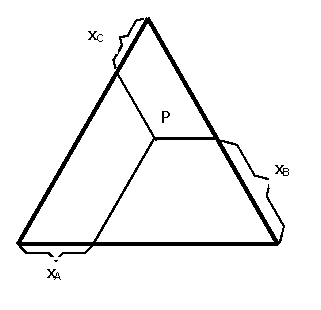
\includegraphics{fig/terner1.eps}
\caption{Composition of a ternary system on a ternary diagram. The mole fraction of the components increases couter-clockwise.}
\label{fig:1}
\end{figure}

Point \emph{,,P''} inside the triangle represents a system with all three components. We can read the composition by finding the respective molefraction values on the axes. The sides give the composition of the pairwise two-component systems as well (Fig. \ref{fig:2} I.). In Fig. \ref{fig:2}. (I.) we show the composition of a ternary system, in which two components mix partially (water--chloroform), while the third (acetic acid for instance) dissolves completely in both. The area below the curve marks the heterogeneous systems. In such a state, the system will have two, so-called \emph{,,conjugated phases''}. Any point in the triangle outside of this area represents a homnogeneous system. Where the curve intersects any side of the triangle, the system has two components; x$_{A,1}$ and x$_{C,1}$ mean the solubility of water in chloroform, x$_{A,2}$ and x$_{C,2}$ mean the solubility of chloroform in water, if A is water, B is acetic acid and C is chloroform. If all the component pairs are only partially soluble in each other, then we get a diagram similar to Fig. \ref{fig:2}. (II.).

\begin{figure}
\centering
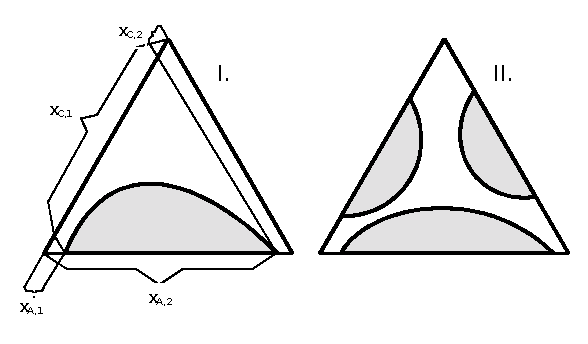
\includegraphics{fig/terner2.eps}
\caption{Phase diagrams of ternary systems. (I.) Only one component pair is partially miscible: the gray area under the curve is heterogeneous, the rest (white area) is homogeneous. (II.) All three component pairs are only partially miscible in each other.}
\label{fig:2}
\end{figure}


From now on we discuss the water--chloroform--acetic acid ternary system. As we have mentioned already, any point below the curve will mean a system with two conjugated phases. Connecting the two points that are representing the conjugated phases we get the so called \emph{,,tie line''}. All the tie lines will have a common intersection, usually outside of the triangle (point \emph{P}, Fig. \ref{fig:3}). The tie lines are usually not parallel with the base of the triangle, because the third component doesn't dissolve equally in the two conjugated phases. Drawing a tangent from pont P to the curve we get point \emph{K}, the \emph{plait point} for a given temperature and pressure. If not all one but two or three component pairs are only partially miscible in each other, the we get two or three plait points, respectively. In the practice we will investigate the water-chloroform-acetic acid ternary system. 

\begin{figure}
\centering
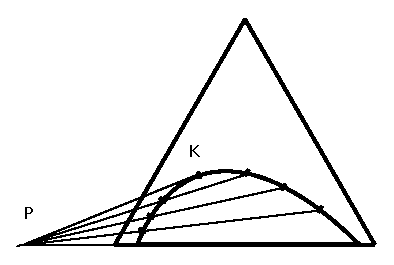
\includegraphics{fig/terner3.eps}
\caption{Determining the plait point in a system in which only one component pair's solubility is limited. P: intersection of the tie lines. K: plait point.}
\label{fig:3}
\end{figure}


\subsection{Practice procedures}

Prepare 20 cm$^3$ 15, 30, 50, 60, 70, 80, 85, 90 and 95 volume\% mixtures of chloroform and acetic acid. The volume\% is given with respect to chloroform. Measure the components with an automatic burette into clean, water-free Erlenmeyer flasks, and close them. Titrate the mixtures with water using a graduated (0.05 cm$^3$) 10 cm$^3$ automatic burette until you observe a slight opaque white color throughout the mixture. Find the density of the components from the table below, and using these and the volumes used until the endpoints (opaque color) calculate the mole fraction and mass fractoin of all three components for all 9 mixtures. Draw the two phase diagrams, using both mole and mass fraction as well (two separate diagrams) to get the equilibrium diagram. Give the results of the calculations in a table such as the following:

\begin{table}[h!]
\centering
\begin{tabular}{|l|l|l|l|l|l|l|l|l|l|l|l|}
\hline
\multicolumn{4}{|c|}{\begin{tabular}[c]{@{}l@{}}organic solvent\\ M = ... g mole$^{-1}$\\ $\rho$ = ... g cm$^{-3}$ \end{tabular}} & \multicolumn{4}{|c|}{\begin{tabular}[c]{@{}l@{}}weak acid\\ M = ... g mole$^{-1}$\\ $\rho$ = ... g cm$^{-3}$ \end{tabular}}  & \multicolumn{4}{|c|}{\begin{tabular}[c]{@{}l@{}}water\\ M = ... g mole$^{-1}$\\ $\rho$ = ... g cm$^{-3}$ \end{tabular}}  \\ \hline
cm$^3$                        & mole                        & x                        & m\%                        & cm$^3$    & mole    & x   & m\%   & cm$^3$   & mole   & x  & m\%  \\ \hline
2                          &                             &                          &                            &        &         &     &       &       &        &    &      \\ \hline
4                          &                             &                          &                            &        &         &     &       &       &        &    &      \\ \hline
...                        &                             &                          &                            &        &         &     &       &       &        &    &      \\ \hline
\end{tabular}
\end{table}


To determine the plate point, prepare a mixture which has two conjugated phases (system under the curve). Separate them, and titrate a known mass of both of them with NaOH to get the mass of acetic acid in both of them. Then calculate the mass fraction of acetic acid in the conjugated phases. After this step we can draw a tie line. Repeat it with another mixture with different composition, to get an additional tie line. Draw a tangent from the intersection of the tie lines to get the plait point. Give the mass fraction composition of this point as a final result of the practice.

Recommendations for the two systems:

\begin{itemize}
\item A: 20 ml water, 25 ml chloroform, 1 ml acetic acid
\item B: 25 ml water, 25 ml chloroform, 3 ml acetic acid
\end{itemize}

Close the flasks, shake them for about 5 minutes to reach equilibrium. Separate the phases in a separation funnel, and titrate 5 ml of the organic and 10 ml of the water phase, after measuring the mass of both. Use either 0.1 M or 1 M NaOH fot titration and a few drops of phenolphthalein as indicator. Prepare the following table:

\begin{table}[h!]
\centering
\begin{tabular}{|l|l|l|l|l|l|}
\hline
phase & \begin{tabular}[c]{@{}l@{}}titrant volume (ml)\\ for organic phase\end{tabular} & m$_{acid}$ (g) & m$_{phase}$ (g) & m\% \\ \hline
A organic      & & & &  \\ \hline
A water        & & & &  \\ \hline
B organic      & & & &  \\ \hline
B water        & & & &  \\ \hline
\end{tabular}
\end{table}


Knowing the mass of the phases you can calculate the mass fraction of acetic acid in both phases. Using these, find the intersection with the equlibrium line to get the conjugated phases' composition. Draw both tie lines. Find point P, the intersection of the tie lines. Draw the tangent to the equilibrium line from point P, to get the plait point K. Read the mass fraction composition of the plait point and write it down in your notebook as a final conclusion.  



\begin{table}[]
\centering
\caption{Solvent molar mass and density.}
\begin{tabular}{rcc}
\multicolumn{1}{l}{}                                & \multicolumn{1}{c}{\begin{tabular}[c]{@{}c@{}}M\\ g mole$^{-1}$\end{tabular}} & \multicolumn{1}{c}{\begin{tabular}[c]{@{}c@{}}Density at 20 $^o$C\\ g cm$^{-3}$\end{tabular}} \\ \hline
\begin{tabular}[c]{@{}r@{}}acetic acid\end{tabular} & 60.05                                                                     & 1.0497                                                                                 \\ \hline
chloroform                                            & 119.38                                                                    & 1.4891                                                                                 \\ \hline
water                                                 & 18.02                                                                     & 0.9982                                                                                
\end{tabular}
\end{table}

%\begin{figure}
%\includegraphics{fig/ternary_diagram.pdf}
%\end{figure}
%\begin{tikzpicture}
%\begin{ternaryaxis}[
%	%title=The water--chloroform--acetic acid ternary system,
%	xlabel=Weight percent of acetic acid,
%	ylabel=Weight percent of chloroform,
%	zlabel=Weight percent of water,
%	label style=sloped,
%	area style,
%]
%	\addplot3 table {
%	0 0.1 0.9
%	 
%	0.28 0.35 0.37
%	0.25 0.6 0.15
%	0.1 0.9 0
%	0 1 0
%	0 0 1
%	};
%	%\addlegendentry{$\gamma$FeNi}
%
%	%\node[inner sep=0.5pt,circle,draw,fill=white,pin=-15:\footnotesize Stainless Steel] at (axis cs:0.18,0.74,0.08) {};
%	
%\end{ternaryaxis}
%\end{tikzpicture}




\newpage
\section{Determination of the composition of a complex by spectrophotometry}
\subsection{Introduction}

The formation of an ML$_n$ complex can be described by the following equilibrium reaction:

\begin{equation}
\text{M} + n\text{L} \rightleftharpoons \text{ML}_n
\end{equation}

As a consequence of the law off mass action, the equilibrium constant of the reaction is defined as follows:

\begin{equation}
K = \frac{[ \text{ML}_n ]}{[ \text{M} ][ \text{L}]^n }
\end{equation}

In this formula, $K$ is the stability product of the complex, [M] is the equilibrium concentration of the free metal ion, [L] is the equilibrium constant of the free ligand, [ML] is the equilibrium concentration of the complex, and $n$ is the number of ligands coordinated to the metal ion.

A common approach to determine the composition of a complex is called Job's method: using solutions of the ligand and the metal that have the same concentrations, a series of samples is prepared in which the sum of these two analytical concentrations is constant, but the ratio varies. (For example, the final volume is always 10 cm$^3$, and a sample is prepared by mixing $x$ cm$^3$ of the ligand solution with $10-x$ cm$^3$ of the metal solution.) It can be proved easily that the sample with the highest concentration of the complex will be the one where the ratio of the ligand and metal ion analytical concentrations is the same as in the complex. 

First, it is noted that the sum of the analytical concentrations of the ligand and the metal is a constant in all the samples:

\begin{equation}
c = c_{\text L} + c_{\text M}
\end{equation}

Differentiating this equation with respect to $c_{\text L}$ gives:

\begin{equation}
0 = 1 + \frac{dc_{\text M}}{dc_{\text L}}
\end{equation}

Simply rearranging this equation gives the following formula for the derivative of  $c_{\text M}$ with respect to  $c_{\text L}$:

\begin{equation}
\frac{dc_{\text M}}{dc_{\text L}} = -1 
\end{equation}

Mass conservation for the metal ion gives:

\begin{equation}
[\text M] = c_{\text M} - [\text {ML}_n] 
\end{equation}

The analogous mass conservation equation for the ligand takes the following form:

\begin{equation}
[\text L] = c_{\text L} - n[\text {ML}_n] 
\end{equation}

Using these mass conservation equation, the equilibrium constant can be written as:

\begin{equation}
K = \frac{[ \text{ML}_n ]}{(c_{\text M} - [\text {ML}_n] )(c_{\text L} - n[\text {ML}_n])^n }
\end{equation}


Differentiating this equation with respect to $c_{\text L}$ gives:

\begin{equation}
\begin{array}{cccc}
0 = K \frac{d[ \text{ML}_n ]}{dc_{\text L}} + \frac{-K}{(c_{\text M} - [\text {ML}_n] )} \left ( -1 - \frac{d[ \text{ML}_n ]}{dc_{\text L}} \right )
\\{}\\
 + \frac{-nK}{(c_{\text L} - n[\text {ML}_n])} \left ( 1 - n \frac{d[ \text{ML}_n ]}{dc_{\text L}} \right )
\end{array}
\end{equation}

At the maximum concentration of the ML$_n$ complex, the derivative $d[ \text{ML}_n ] / dc_{\text L}$ is zero. In the previous equation, this leaves a very simple relationship:

\begin{equation}
0 = \frac{K}{(c_{\text M} - [\text {ML}_n] )}  + \frac{-nK}{(c_{\text L} - n[\text {ML}_n])} 
\end{equation}

This equation can be re-arranged further:

\begin{equation}
n(c_{\text M} - [\text {ML}_n] ) = (c_{\text L} - n[\text {ML}_n]) 
\end{equation}

Finally, it is noted that the term $n[\text {ML}_n]$ occurs on both sides, the ratio of the two analytical concentrations is obtained:

\begin{equation}
\frac{c_{\text L}}{c_{\text M}}= n 
\end{equation}

This line of thought proves that maximum concentration of {ML}$_n$ will be reached in a solution where the ligand-to-metal concentration ratio is exactly $n$, i.e. the stoichiometric value.

If the complex is colored, the ratio at which maximum complex formation occurs can be determined easily and the composition of the complex can be deduced. According to Beer's law, the absorbance ($A$) of a solution at a given wavelength $\lambda$ is given as:

\begin{equation}
A = \epsilon_{\lambda} c l 
\end{equation}

If all three components (M, L and ML$_n$) have absorptions, three terms need to be given in this equation:

\begin{equation}
A = (\epsilon_{\text M} [\text M] +\epsilon_{\text L} [\text L] + \epsilon_{\text {ML}_n} [\text {ML}_n])l 
\end{equation}

The molar absorbances of all species appear in this equation. In the absence of any complex formation, the expectation for the absorbance would be:

\begin{equation}
A' = \epsilon_{\text M} (c - c_{\text L}) l +\epsilon_{\text L} c_{\text L} l 
\end{equation}
 
The difference between $A$ and $A'$ can be expressed taking the mass conservation equations into account:

\begin{equation}
\begin{array}{cccc}
A - A' = \epsilon_{\text M} (c - c_{\text L} - [\text {ML}_n]) l + \epsilon_{\text L} (c_{\text L} - n[\text {ML}_n]) l + \epsilon_{\text {ML}_n} [\text {ML}_n] l
\\{}\\
 - \epsilon_{\text M} (c - c_{\text L}) l - \epsilon_{\text L} c_{\text L} l =
\\{}\\
(\epsilon_{\text {ML}_n} - \epsilon_{\text M} - n \epsilon_{\text L}) [\text {ML}_n] 
\end{array}
\end{equation}

Because of this direct proportionality, it is clear that $A-A'$ will have an extremum exactly where $[\text {ML}_n]$ has. Therefore, the absorbance signal can be used for the determination of the composition of the complex.



\subsection{Practice procedures}

Ask your instructor which metal ion ligand pair you should do experiments on. Prepare 100 cm$^3$  20-fold dilutions of both of the stock solutions, then prepare the samples given in the following table:


\begin{table}[H]
\centering
\caption{Composition of individual experiments}
\begin{tabular}{|c|c|c|c|c|c|}
\hline
Sample& M & L & Sample  & M & water  \\

number & cm$^3$ & cm$^3$ & number & cm$^3$ & cm$^3$ \\

\hline
1 & 1.0 & 9.0 & 1' & 1.0 & 9.0 \\

\hline
2 & 2.0 & 8.0 & 2' & 2.0 & 8.0 \\

\hline
3 & 3.0 & 7.0 & 3' & 3.0 & 7.0 \\

\hline
4 & 4.0 & 6.0 & 4' & 4.0 & 6.0 \\

\hline
5 & 5.0 & 5.0 & 5' & 5.0 & 5.0 \\

\hline
6 & 6.0 & 4.0 & 6' & 6.0 & 4.0 \\

\hline
7 & 7.0 & 3.0 & 7' & 7.0 & 3.0 \\

\hline
8 & 8.0 & 2.0 & 8' & 8.0 & 2.0 \\

\hline
9 & 9.0 & 1.0 & 9' & 9.0 & 1.0 \\

\hline

\end{tabular}
\end{table}

Put the samples in the first series on white paper and select the one that has the most intense color. Fill a cuvette with 1.000 cm path length with this solution and record its spectrum in the visible range (370-650 nm) using water as a reference. Select the wavelength at which the absorbance is the highest (this is called the peak in the spectrum). Measure the absorbances of all other solutions at this wavelength. Measure the absorbances of all samples in the second series at the same wavelength. Finally, record the absorption spectrum of the metal ion solution using the original (undiluted) stock solution of the metal

\subsection{Evaluation}

Draw the two absoprtion spectra (i.e. that of the complex and that of the metal ion). At the selected wavelength, give the measured absorbance values in a table:


\begin{table}[H]
\centering
\begin{tabular}{|c|c|c|c|c|}
\hline
Sample & L & $A$ & $A'$ & $A-A'$ \\

Number   & (cm$^3$) &  &  &  \\

\hline
1 &   &   &   &    \\

\hline
2 &   &   &  &    \\

\hline
... &   &   &  &   \\

\hline
\end{tabular}
\end{table}

Plot the $A-A'$ values as a function of the ligands solution volume used (in cm$^3$), determine where the maximum occurs and deduce the composition of the complex.

\newpage
\documentclass{article}
\usepackage{amsmath}
\usepackage{amssymb}
\usepackage{gensymb}
\usepackage{upgreek}
\usepackage{float}
\usepackage{graphicx}

\begin{document}

\begin{figure}
  \centering
  \includegraphics[width=0.3\textwidth]{labsafety.jpg}
\end{figure}

\title{Safety Instructions and General Guide for the Physical Chemistry Laboratory Practice of Pharmacy Students}
\author{Andr\'{a}s Kiss, assistant lecturer}
%Department of General and Physical Chemistry, Faculty of Sciences, University of P\'{e}cs, 7624 P\'{e}cs, Ifj\'{u}s\'{a}g \'{u}tja 6, Hungary
\date{September 2015}
\maketitle
%\address[akiss, gnagy]{J\'{a}nos Szent\'{a}gothai Research Centre, University of P\'{e}cs, 7624 P\'{e}cs, Ifj\'{u}s\'{a}g \'{u}tja 20, Hungary}
%\ead{akiss@gamma.ttk.pte.hu}

Working in a chemistry laboratory can be dangerous. You are exposed to a wide range of chemicals, flame, high temperature devices ie. hotplate, high pressure containers, sharp tools, fragile glassware. Safe laboratory practice is essential to prevent any injure in yourself, and others.

First and foremost, you should always be prepared for your current laboratory practice. You should be familiar with the topic. Prepare for the practice in advance. Depending on the subject spend at least 1 to 2 hours with preparations by studying the handout carefully in the day before the pactice, and about 15 minutes before the practice. Understand the task at hand. If you don't know what you are doing, you will make mistakes, unnecessarily prolong the practice, endanger yourself and others, and ultimately fail. With good preparation however, the practice will be useful, succesful, and even fun.

\begin{enumerate}
\item You may carry to the laboratory only the following items:
	\begin{itemize}
	\item your notebook,
	\item pen,
	\item marker,
	\item calculator,
	\item labcoat,
	\item your own spatula if you have one.
	\end{itemize}
\item You may NOT carry these to the laboratory:
	\begin{itemize}
	\item food,
	\item drinks,
	\item your bag,
	\item jacket,
	\item umbrella.
	\end{itemize}
\item You may NOT do these in the laboratory:
	\begin{itemize}
	\item eat,
	\item drink,
	\item smoke,
	\item do any other practice than your own,
	\item be alone in the laboratory.
	\end{itemize}
\end{enumerate}

Always wait for the supervising teacher to arrive before you enter the laboratory. Be punctual, arrive at least 5 minutes before the practice starts, at the entrance, ready for the work. Leave your bag, jacket, umbrella etc. in your locker at the designated area. Do not leave anything at the entrance.
	
Start your work by cleaing your work area. Then wash everything (eg. glassware, electrodes, cuvettes, beakers, flasks, spatulas, pipettes, burettes) first by tapwater, use detergents and scrubber if necessary. Then, flush it with ionized water, or double ionized water, depending on the requirements of the practice. For example to determine the solubility product of a sparingly soluble salt, both the electrodes, and the glassware have to be extremely clean. Wash glassware with great care for these practices. The quality of your work will depend on your effectiveness of cleaning.

It is VERY important to write down everything you do in the laboratory. A short guide about this can be found in the foreword of your practice handouts. Precise record keeping is essential for the evaluation of your work. Write down your observations, measured data, the precise time if possible, and even the results of unsuccesful work. These might turn out to be "succesful" experiments later.

Always label every solution you prepare with a marker. If you are unsure about the content of an unlabeled container, don't use it! Use only labeled chemicals. It is strongly advised to bring your own marker to the practice instead of constantly keep borrowing someone else's.

Never use broken equipment. If you notice a crack or even the smallest one, dispose it in the designated waste container. Always notify the laboratory supervisor about broken equipment.

Dispose aqeous solutions with low environmental hazard into the sink. Use excess water to wash it down. Neutralize concentrated acids and bases before disposing. There is an organic solvent waste located below the fume hood. You may dispose organic waste into this container only. Do not throw solids in the sink eg. pieces of broken glass, spatulas. Do not pour fluids into the sink if there is a magnetic stirrer in it. Remove the stirrer first.

Use protective equipment if necessary. Latex gloves and  safety glasses will be in your drawer. Always wear your labcoat during the entire practice. It is advised to button your coat. Do not wear open shoes. Keep your hair up.

Do not smell chemicals directly. Use your hands as a fan instead to smell the chemical. Do not taste any chemical under any circumstances! If a chemical is accidentally swallowed, wash it with excessive water, and notify the supervisor immediately!

We won't use open flame during this practice. If there is a fire however, you can find fire extinguishers in the lab, and in the corridor. There is an emergency shower located above the door in the laboratory. Use this immediately if your cloth catches on fire. Stand below the shower, and pull the lever. The elevators may not be used during a fire alarm. In case of a fire alarm, use the emergency stairs ti exit the building.

Fire will persist of there is flammable material, enough oxygen, and high enough temperature. Remove any of these, and the fire will stop. The building has an automatic ventillation system, the windows cannot be opened. You can cover the fire with a blanket or a piece of wet clothing to prevet oxygen resupply to the fire. Depending on the fire, use different fire extinguishers. To extinguish electric fire, do not use water based extinguishers! Use only dry chemical extinguiser in these cases.

There is a first aid kit in the laboratory to provide basic medical assistance. If acids or bases are spilled on your skin, use plenty of water to wash it, then use 2\% sodium-hydroge-carbonate and 2\% acetic acid for injuries caused by acids and bases, respectively. If these are spilled into your eyes, use 2\% sodium-borate (borax), and 2\% boric-acid for acids and bases, respectively, after washing it with plenty of water. 

In case of gas intoxication, get fresh air immediately. As the windows are not openable in our laboratory, you should get out of the building immediately accompanied by at least two other persons. Notify the ambulance in any case of intoxication or injury! Use fume hood for the practices using volatile chemicals (chloroform, cc. acetic-acid). If acid is swallowed, DO NOT swallow sodium-carbonate to neutralize it, as a huge amount of carbon-dioxide could potentially evolve, and the injures stomach might rupture. In case of electrical shock, notify the supervisor, and seek medical assistance immediately!


\begin{figure}
  \centering
  \includegraphics[width=1\textwidth]{old_hazard.png}
  \caption{Old chemical hazard symbols.}
\end{figure}


\begin{figure}
  \centering
  \includegraphics[width=1\textwidth]{new_hazard.png}
  \caption{New chemical hazard symbols.}
\end{figure}

\end{document}

\newpage
\fancyhead[LE,RO]{Appendix A -- Ionic conductivity at infinite dilution}
\fancyhead[LO,RE]{\thesection}
\fancyfoot[LE,RO]{\thepage}
\fancyfoot[RE,LO]{\emph{Physical chemistry lab. practice for pharmacy students}}

\section*{Appendix A -- Ionic conductivity at infinite dilution}
\addcontentsline{toc}{section}{Appendix A -- Ionic conductivity at infinite dilution}
The following table includes the molar ionic conductivities at infinite dilution for certain ions, that are necessary for evaluations in certain practices. The values refer to aqueous solutions at 25 $\celsius$.

\begin{table}[h!]
\centering
\caption{Molar ionic conductivity at infinite dilution. Source: CRC Handbook of Chemistry and Physics 76th edition, David R. Lide editor in chief, 1995-1996 ISBN: 0-8493-0476-8.}
\label{table:conductivities}
\vspace{5mm}
\begin{tabular}{l|c}
%\hline
                        Ion \hspace{2cm} & $\lambda^0_\pm$, $\cdot$10$^{-4}\cdot$m$^2 \cdot$S$\cdot$mol$^{-1}$\\
                      \hline


Ag$^+$ \dotfill & 61.9 \\
1/3 Al$^{3+}$ \dotfill& 61 \\
1/2 Ba$^{2+}$\dotfill& 63.6 \\
1/2 Be$^{2+}$\dotfill& 45 \\
1/2 Ca$^{2+}$\dotfill& 59.47 \\
1/2 Cd$^{2+}$\dotfill& 54 \\
1/3 Ce$^{3+}$\dotfill& 69.8 \\
1/2 Co$^{2+}$\dotfill& 55 \\
%1/3 [Co(NH$_3$)$_6$]$^{3+}$\dotfill& \\
%1/3 [Co(en)$_3$]$^{3+}$\dotfill& \\
%1/6 [Co$_2$(trien)$_3$]$^{6+}$\dotfill& \\
%1/3 Cr$^{3+}$\dotfill& \\
%Cs$^+$\dotfill& \\
1/2 Cu$^{2+}$\dotfill& 69.3 \\
%D$^+$\dotfill& \\
%1/3 Dy$^{3+}$\dotfill& \\
%1/3 Er$^{3+}$\dotfill& \\
%1/3 Eu$^{3+}$\dotfill& \\
1/2 Fe$^{2+}$\dotfill& 54 \\
1/3 Fe$^{3+}$\dotfill& 68 \\
%1/3 Gd$^{3+}$\dotfill& \\
H$^+$\dotfill& 67.3 \\
1/2 Hg$^{2+}$\dotfill& 68.6 \\
%1/2 Hg$^{2+}$\dotfill& \\
%1/3 Ho$^{3+}$\dotfill& \\
K$^+$\dotfill& 73.48 \\
%1/3 La$^{3+}$\dotfill& \\
%Li$^+$\dotfill& \\
1/2 Mg$^{2+}$\dotfill& 53.0 \\
%1/2 Mn$^{2+}$\dotfill& \\
%NH$_4^{+}$\dotfill& \\
%N$_2$H$_5^+$\dotfill& \\
1/2 CO$_3^{2-}$\dotfill & 69.3 \\

\end{tabular}
\end{table}


\end{document}
